
\section{Representaciones para una palabra}

Hasta ahora, básicamente hemos tenido una representación de las palabras, las incrustaciones de palabras que ya hemos aprendido: Word2vec, GloVe, fastText. Estas incrustaciones tienen una calidad semi-supervisada útil, ya que se pueden aprender a partir de corpora no etiquetados y se utilizan en nuestras arquitecturas orientadas a tareas posteriores (LSTM, CNN, Transformer).

Sin embargo, presentan dos problemas. El problema 1 es que siempre producen la misma representación para un tipo de palabra, independientemente del contexto en el que se encuentre un token de palabra. Podríamos querer una desambiguación muy precisa del sentido de las palabras. El problema 2 es que solo tenemos una representación para una palabra, pero las palabras tienen diferentes aspectos, incluyendo la semántica, el comportamiento sintáctico y el registro/connotaciones.

\section{Los Modelos de Lenguaje Neurales pueden producir Incrustaciones Contextualizadas}

En un Modelo de Lenguaje Neural (MLN), introducimos inmediatamente vectores de palabras (tal vez solo entrenados en el corpus) a través de capas LSTM. Estas capas LSTM se entrenan para predecir la siguiente palabra. Sin embargo, estos modelos de lenguaje producen representaciones de palabras específicas del contexto en los estados ocultos de cada posición.

\begin{figure}[h]
  \centering
  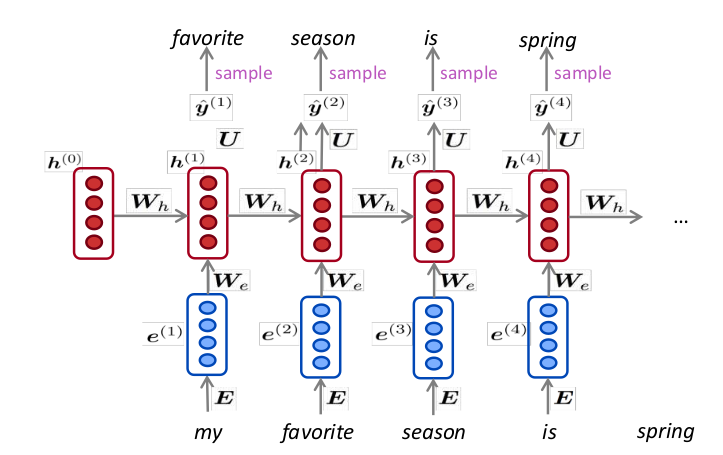
\includegraphics[scale=0.4]{pics/lstm_nlm.png}
  \caption{Modelo de Lenguaje Neural con capas LSTM}
\end{figure}

\section{ELMo: Incrustaciones de Modelos de Lenguaje}

La idea detrás de ELMo es entrenar un modelo de lenguaje grande (LM) con una red neuronal recurrente y utilizar sus estados ocultos como "incrustaciones de palabras contextualizadas" \cite{peters-etal-2018-deep}. ELMo es un modelo de lenguaje bidireccional con 2 capas de biLSTM y alrededor de 100 millones de parámetros. Utiliza una CNN de caracteres para construir la representación inicial de las palabras. Utiliza 2048 filtros de n-gramos de caracteres y 2 capas de paso alto, con una proyección de 512 dimensiones. Utiliza estados LSTM ocultos/celdas de 4096 dimensiones con proyecciones de 512 dimensiones para la siguiente entrada. Utiliza una conexión residual y los parámetros de la entrada de token y la salida (softmax) están ligados.

\begin{figure}[h]
  \centering
  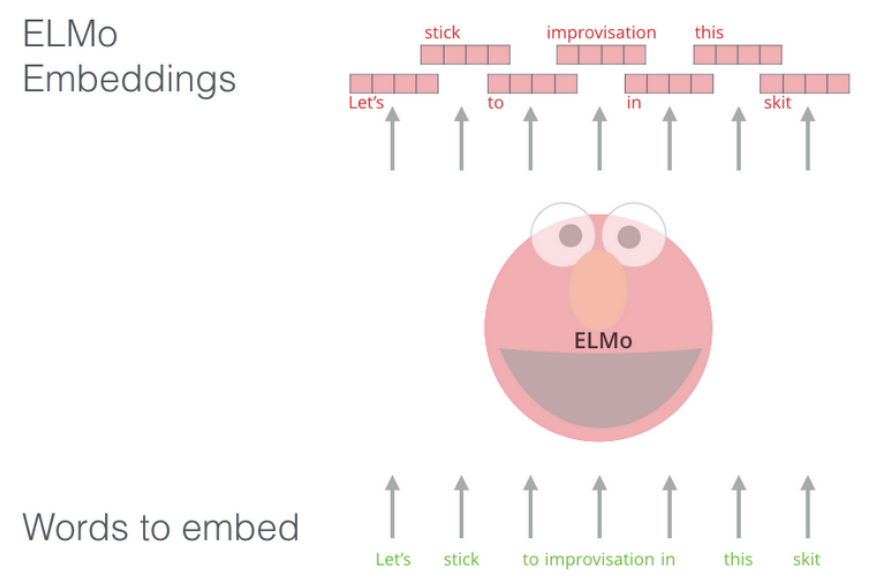
\includegraphics[scale=0.29]{pics/elmo.png}
  \caption{Arquitectura de ELMo}
\end{figure}

\subsection{ELMo: Uso con una tarea}

El primer paso es ejecutar el modelo de lenguaje bidireccional para obtener representaciones para cada palabra. Luego, el modelo de tarea específica puede utilizar estas representaciones. Se congelan los pesos de ELMo con fines de modelo supervisado y se concatenan los pesos de ELMo en el modelo específico de la tarea.

\begin{figure}[h]
  \centering
  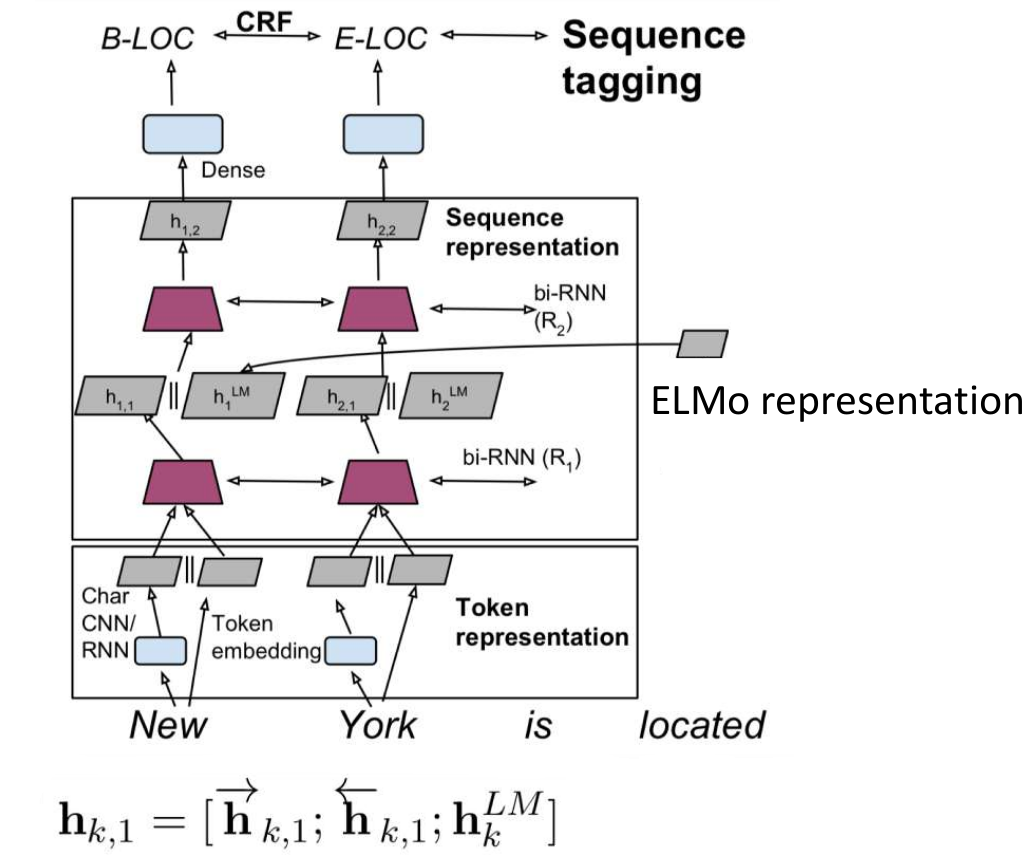
\includegraphics[scale=0.25]{pics/elmo2.png}
  \caption{Uso de ELMo en una tarea específica}
\end{figure}

\paragraph{ELMo: Resultados}

\begin{figure}[h]
  \centering
  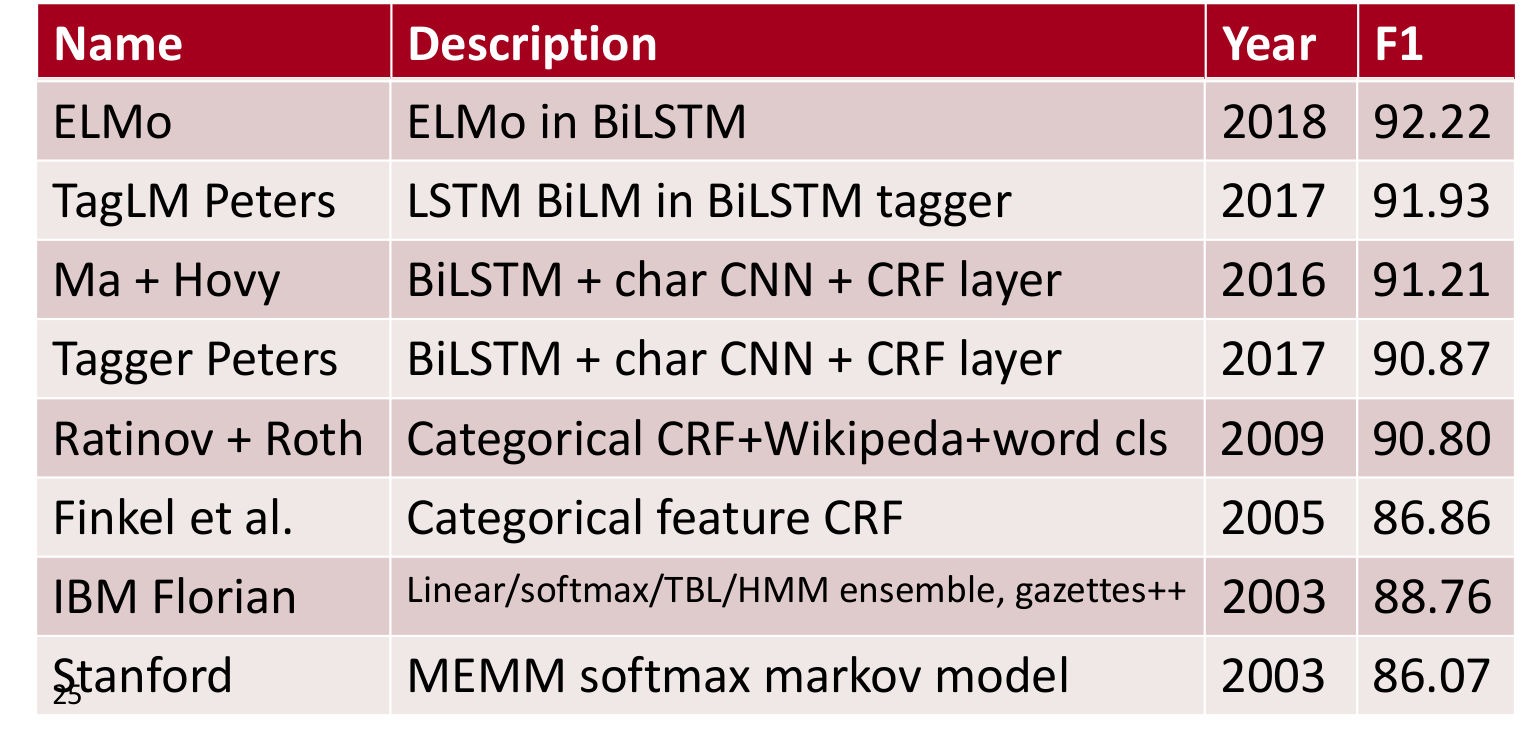
\includegraphics[scale=0.25]{pics/elmo_results.png}
  \caption{Resultados de ELMo en diferentes tareas}
\end{figure}

\section{ULMfit}

Howard y Ruder (2018) propusieron Universal Language Model Fine-tuning (ULMfit) para la clasificación de texto \cite{howard-ruder-2018-universal}. La idea general es transferir el conocimiento de un modelo de lenguaje a la tarea específica. En ULMfit, se entrena un modelo de lenguaje en un corpus grande y general y luego se ajusta en los datos de la tarea objetivo. Finalmente, se utiliza el modelo ajustado como clasificador en la tarea objetivo.

\begin{figure}[h]
  \centering
  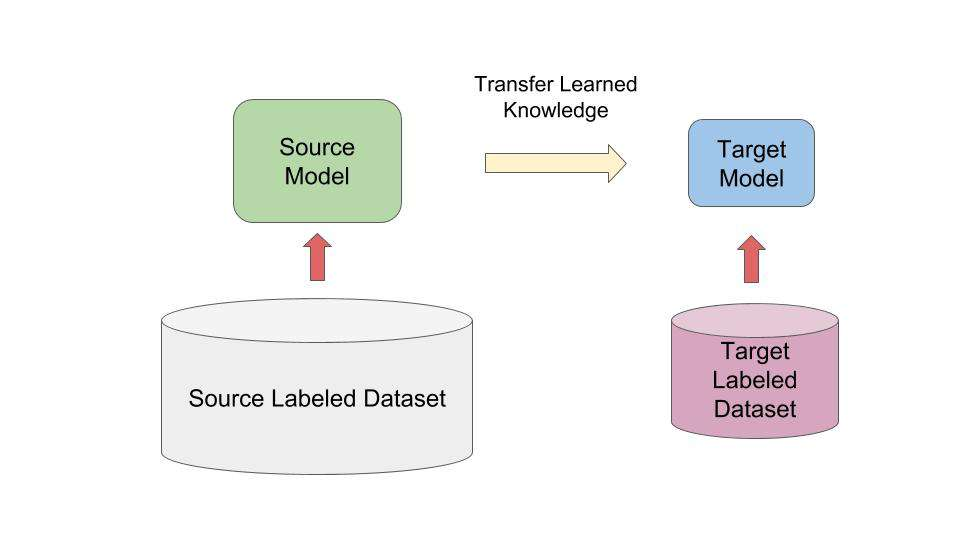
\includegraphics[scale=0.29]{pics/ulmfit1.png}
  \caption{ULMfit: Ajuste fino de un modelo de lenguaje}
\end{figure}

\subsection{Énfasis de ULMfit}

ULMfit utiliza un modelo de lenguaje de "1 GPU" de tamaño razonable, en lugar de uno enorme. Se presta mucha atención al ajuste fino del modelo de lenguaje, con tasas de aprendizaje diferentes por capa, un programa de aprendizaje con tasas de aprendizaje triangular y un descongelamiento gradual de capas y programación de tasas de aprendizaje triangular al aprender el clasificador. Para la clasificación, se utiliza la concatenación de los estados $h_T$, maxpool$(h)$ y meanpool$(h)$.

\begin{figure}[h]
  \centering
  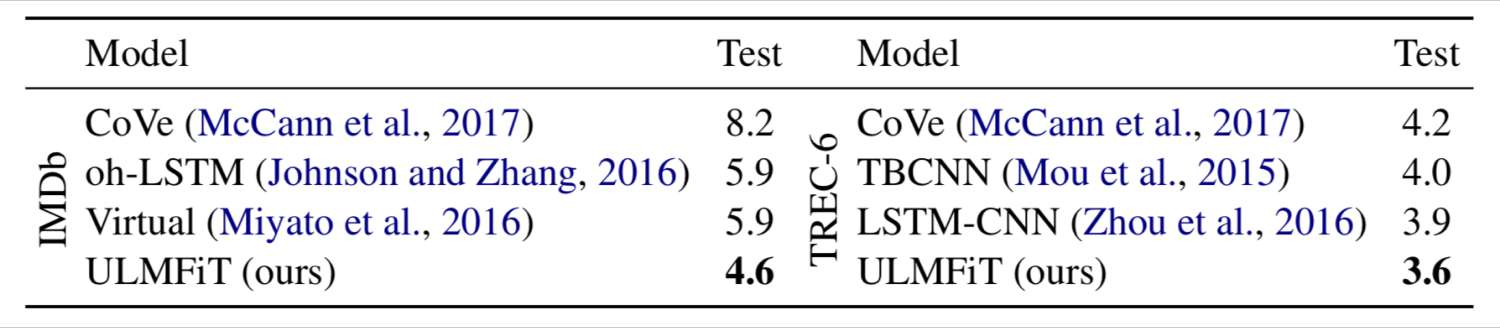
\includegraphics[scale=0.2]{pics/ulmfit3.png}
  \caption{Tasas de error de clasificación de un clasificador de texto}
\end{figure}

\subsection{Transferencia de aprendizaje con ULMfit}

\begin{figure}[h]
  \centering
  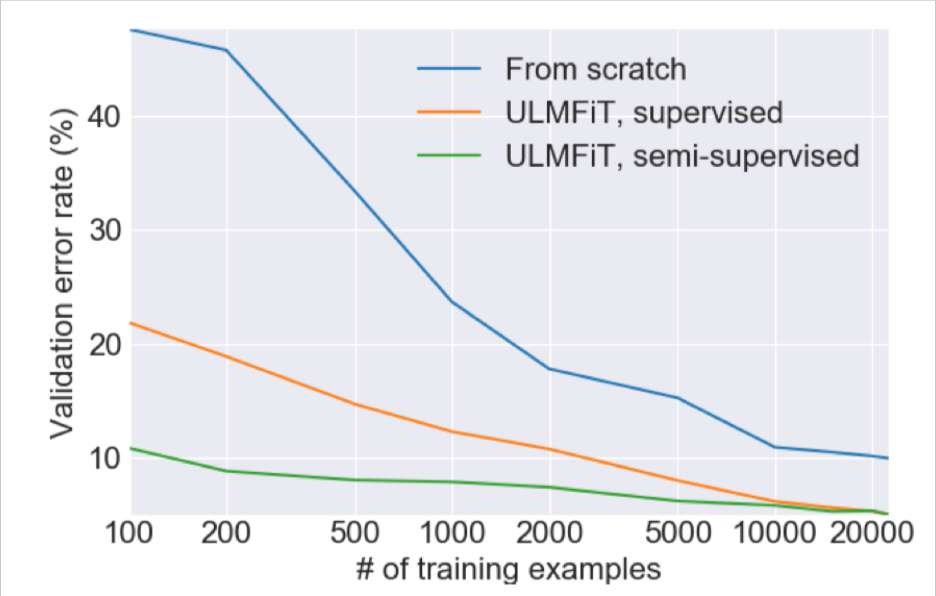
\includegraphics[scale=0.3]{pics/ulmfit4.png}
  \caption{Transferencia de aprendizaje con ULMfit}
\end{figure}

\section{¡Aumentemos la escala!}

\begin{figure}[h]
  \centering
  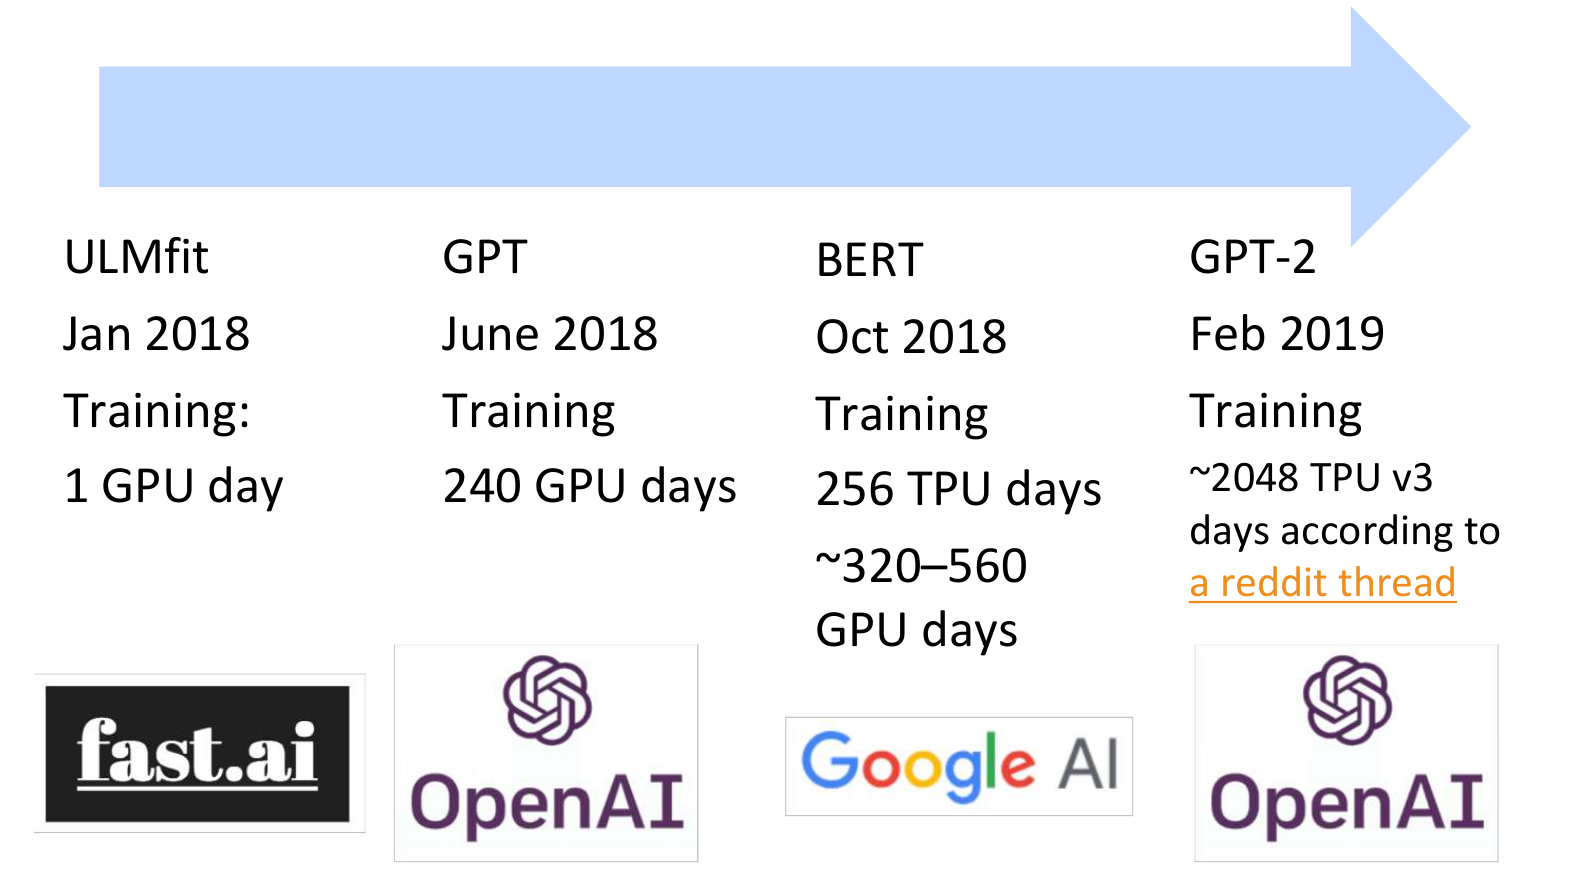
\includegraphics[scale=0.28]{pics/llmscale.png}
  \caption{Aumentando la escala de los modelos de lenguaje grandes}
\end{figure}

\begin{figure}[h]
  \centering
  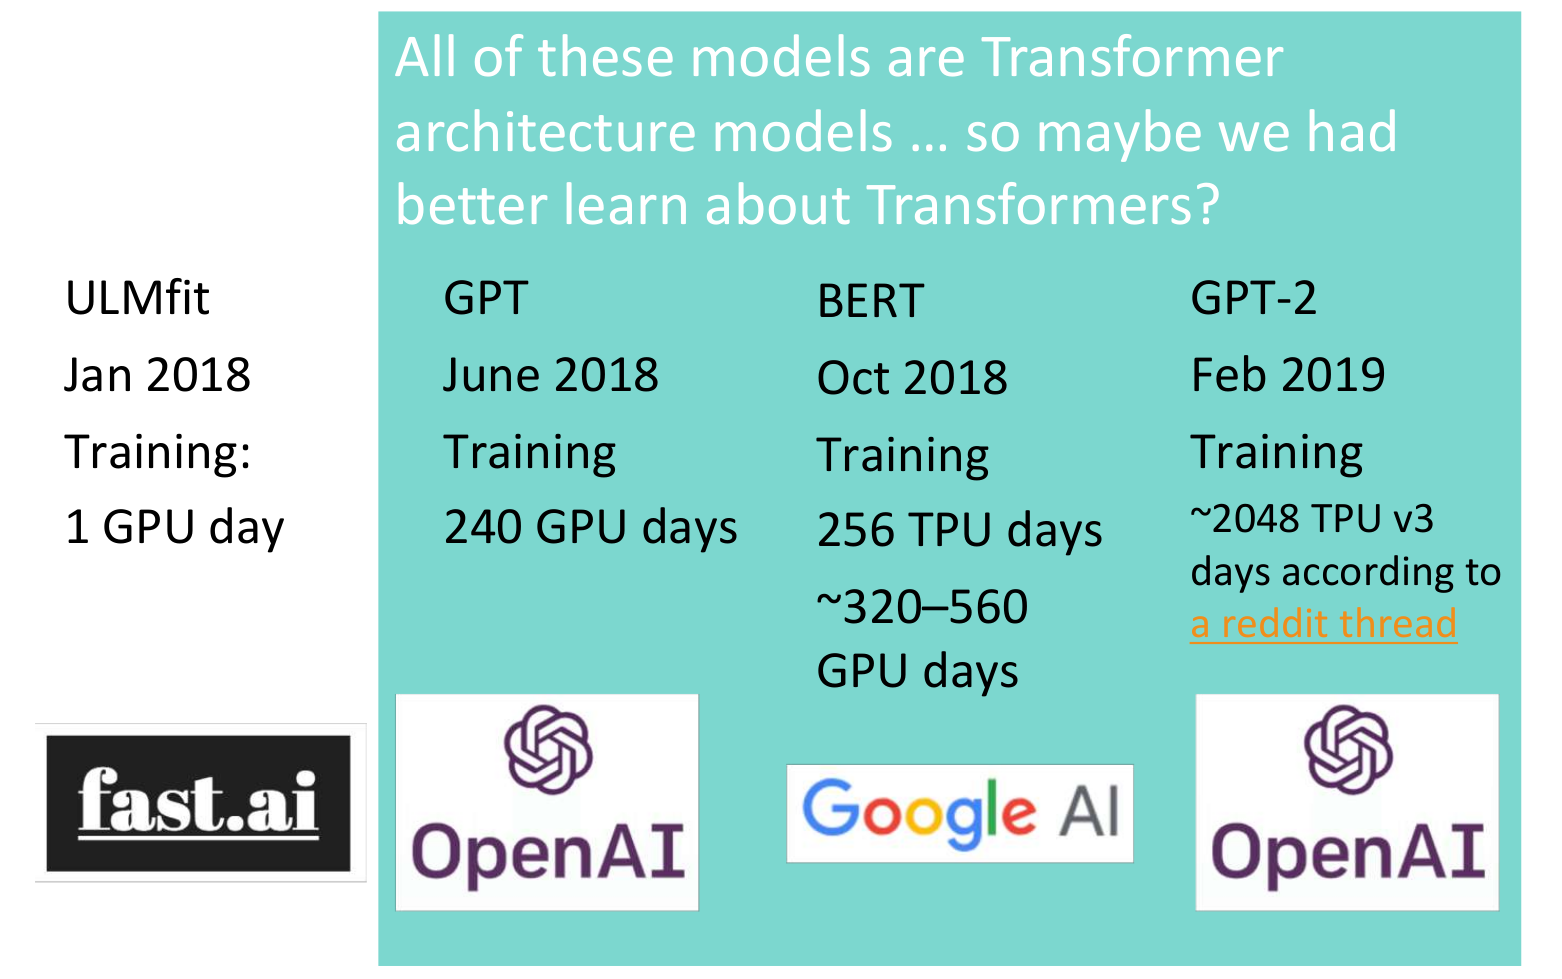
\includegraphics[scale=0.28]{pics/llmscale_trans.png}
  \caption{Evolución de los modelos de lenguaje grandes}
\end{figure}

\section{BERT (Bidirectional Encoder Representations from Transformers)}

La idea detrás de BERT es combinar ideas de ELMO, ULMFit y el Transformer \cite{kenton2019bert}. BERT es un modelo grande (335 millones de parámetros) entrenado a partir de un corpus no etiquetado utilizando un codificador Transformer y luego se ajusta en otras tareas posteriores.

Las propiedades paralelizables del Transformer permiten que el modelo se escale a más parámetros, a diferencia de las RNN, que deben procesarse secuencialmente. BERT no predice la siguiente palabra en una oración como un modelo de lenguaje tradicional, sino que utiliza un objetivo de "modelado de lenguaje enmascarado" (MLM) durante el preentrenamiento.

En MLM, se enmascaran palabras aleatorias en una oración y el modelo se entrena para predecir esas palabras enmascaradas en función del contexto circundante. BERT también incorpora una tarea de "predicción de la siguiente oración", donde se alimentan pares de oraciones al modelo y aprende a predecir si la segunda oración sigue a la primera en el texto original.

Para el ajuste fino de BERT, se agrega una capa específica de la tarea sobre el modelo preentrenado y se entrena en un conjunto de datos etiquetados para la tarea objetivo. BERT logró resultados de vanguardia en el momento de su lanzamiento en tareas de procesamiento del lenguaje natural, incluyendo clasificación de oraciones, reconocimiento de entidades nombradas, respuestas a preguntas y más.

\section{Modelado de Lenguaje Mascarado y Predicción de la Siguiente Oración}

MLM implica enmascarar k\% de las palabras de entrada y luego predecir las palabras enmascaradas. Usualmente, se utiliza k = 15\%. Si se enmascaran muy pocas palabras, el entrenamiento se vuelve muy costoso. Si se enmascaran demasiadas palabras, se pierde contexto suficiente.

La predicción de la siguiente oración se utiliza para aprender las relaciones entre las oraciones. El modelo intenta predecir si la oración B es la siguiente en el texto original después de la oración A, o si es una oración aleatoria.

\section{Codificación de pares de oraciones en BERT}

BERT utiliza incrustaciones de tokens para representar palabras. Las palabras se dividen en unidades más pequeñas llamadas "word pieces" y cada "word piece" se asigna a una incrustación de token. BERT aprende una incrustación segmentada [SEP] para diferenciar entre las dos oraciones en un par. También utiliza incrustaciones posicionales para capturar la posición de cada palabra dentro de la oración.

\section{Arquitectura y entrenamiento del modelo BERT}

BERT se basa en el codificador Transformer. El bloque de atención propia de múltiples cabezas del Transformer permite a BERT considerar el contexto a larga distancia de manera efectiva. El uso de la atención propia también permite cálculos eficientes en GPU/TPU, con solo una multiplicación por capa. BERT se entrenó en una gran cantidad de datos de texto no etiquetado de Wikipedia y BookCorpus. Se entrenaron dos tamaños de modelo diferentes:

\begin{enumerate}
\item BERT-Base: 12 capas, 768 unidades ocultas y 12 cabezas de atención.
\item BERT-Large: 24 capas, 1024 unidades ocultas y 16 cabezas de atención.
\end{enumerate}

El proceso de entrenamiento involucró el uso de configuraciones de TPU (Tensor Processing Unit) 4x4 o 8x8 para una computación más rápida. El entrenamiento de los modelos BERT tomó aproximadamente 4 días para completarse.

\section{Ajuste fino del modelo BERT}

El ajuste fino implica personalizar el modelo preentrenado de BERT para tareas específicas. Para el ajuste fino de BERT, se agrega una capa específica de la tarea sobre el modelo preentrenado de BERT. La capa específica de la tarea puede variar según la tarea en cuestión, como el etiquetado de secuencias o la clasificación de oraciones. Se entrena el modelo completo, incluido el modelo preentrenado de BERT y la capa específica de la tarea, para la tarea específica.

\begin{figure}[h]
  \centering
  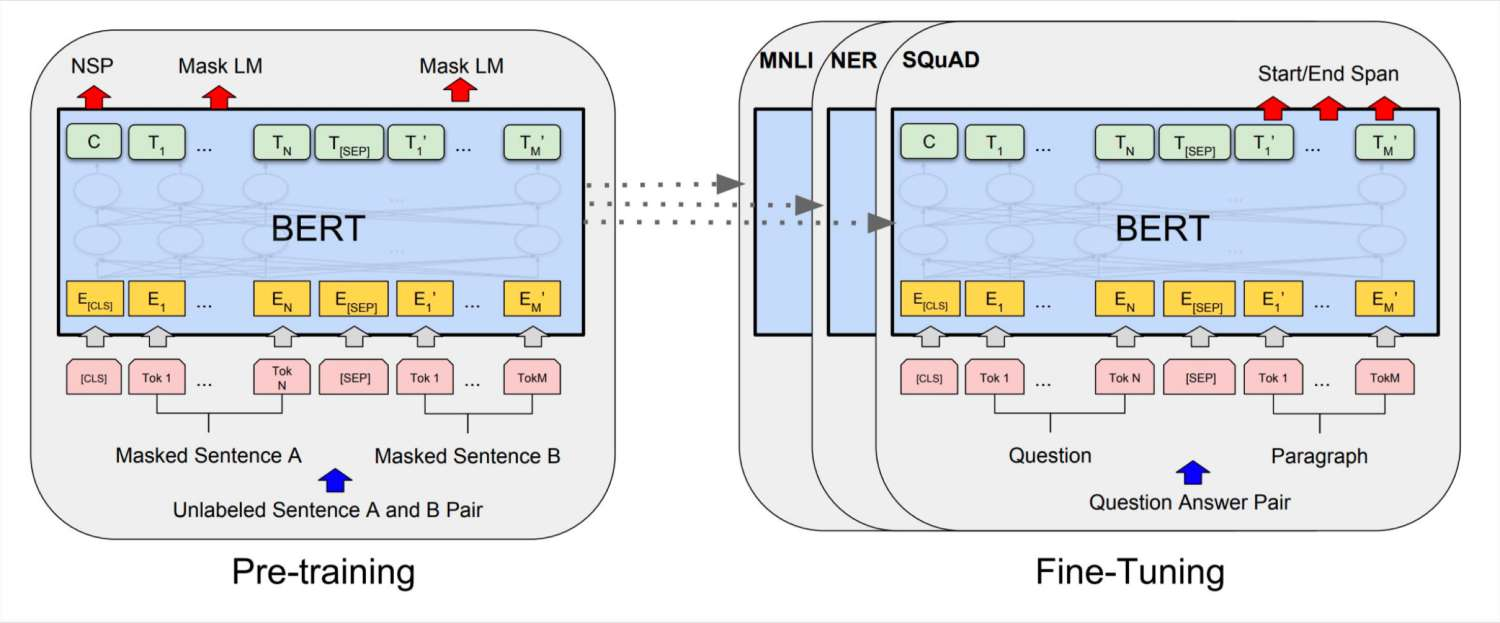
\includegraphics[scale=0.2]{pics/BERTFineTuning.png}
  \caption{Ajuste fino del modelo BERT}
\end{figure}

\subsection{Resultados de BERT en tareas GLUE}

BERT fue extremadamente popular y versátil, y el ajuste fino de BERT condujo a nuevos resultados de vanguardia en una amplia gama de tareas. El rendimiento de BERT se evaluó utilizando el benchmark GLUE, una colección de diversas tareas de procesamiento del lenguaje natural. El benchmark GLUE consiste principalmente en tareas de inferencia de lenguaje natural, pero también incluye tareas de similitud de oraciones y análisis de sentimientos.

\paragraph{Tareas de GLUE}
\begin{itemize}
\item QQP: Quora Question Pairs (detectar preguntas parafraseadas)
\item QNLI: inferencia de lenguaje natural sobre datos de respuesta a preguntas
\item SST-2: análisis de sentimientos
\item CoLA: corpus de aceptabilidad lingüística (detecta si las frases son gramaticales.)
\item STS-B: similitud semántica textual
\item MRPC: corpus de paráfrasis de Microsoft
\item RTE: pequeño corpus de inferencia en lenguaje natural
\end{itemize}


Ejemplo de tarea: MultiNLI (Inferencia de lenguaje natural)
\begin{itemize}
\item Premisa: "Las colinas y montañas son especialmente sagradas en el jainismo."
\item Hipótesis: "El jainismo odia la naturaleza."
\item Etiqueta: Contradicción
\end{itemize}

Ejemplo de tarea: CoLa
\begin{itemize}
\item Oración: "La carreta resonó por el camino."
\item Etiqueta: Aceptable
\end{itemize}
\begin{itemize}
\item Oración: "El automóvil tocó la bocina por el camino."
\item Etiqueta: Inaceptable
\end{itemize}

\begin{figure}[h]
  \centering
  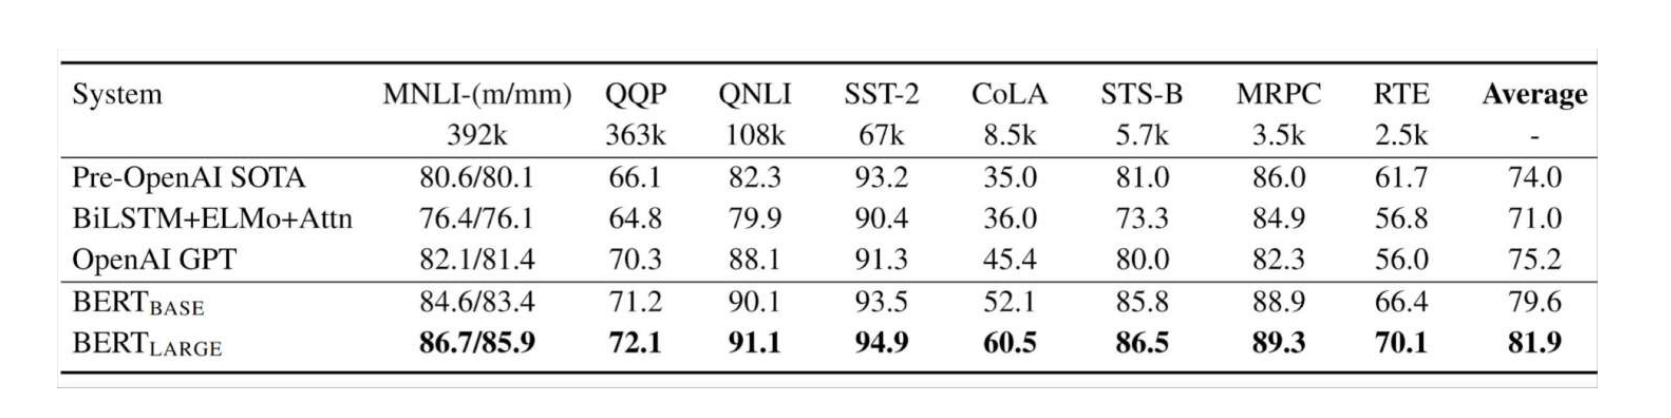
\includegraphics[scale=0.26]{pics/BERTGLUE.png}
  \caption{Resultados de BERT en tareas GLUE}
\end{figure}

\subsection{Efecto de la tarea de preentrenamiento en BERT}

\begin{figure}[h]
  \centering
  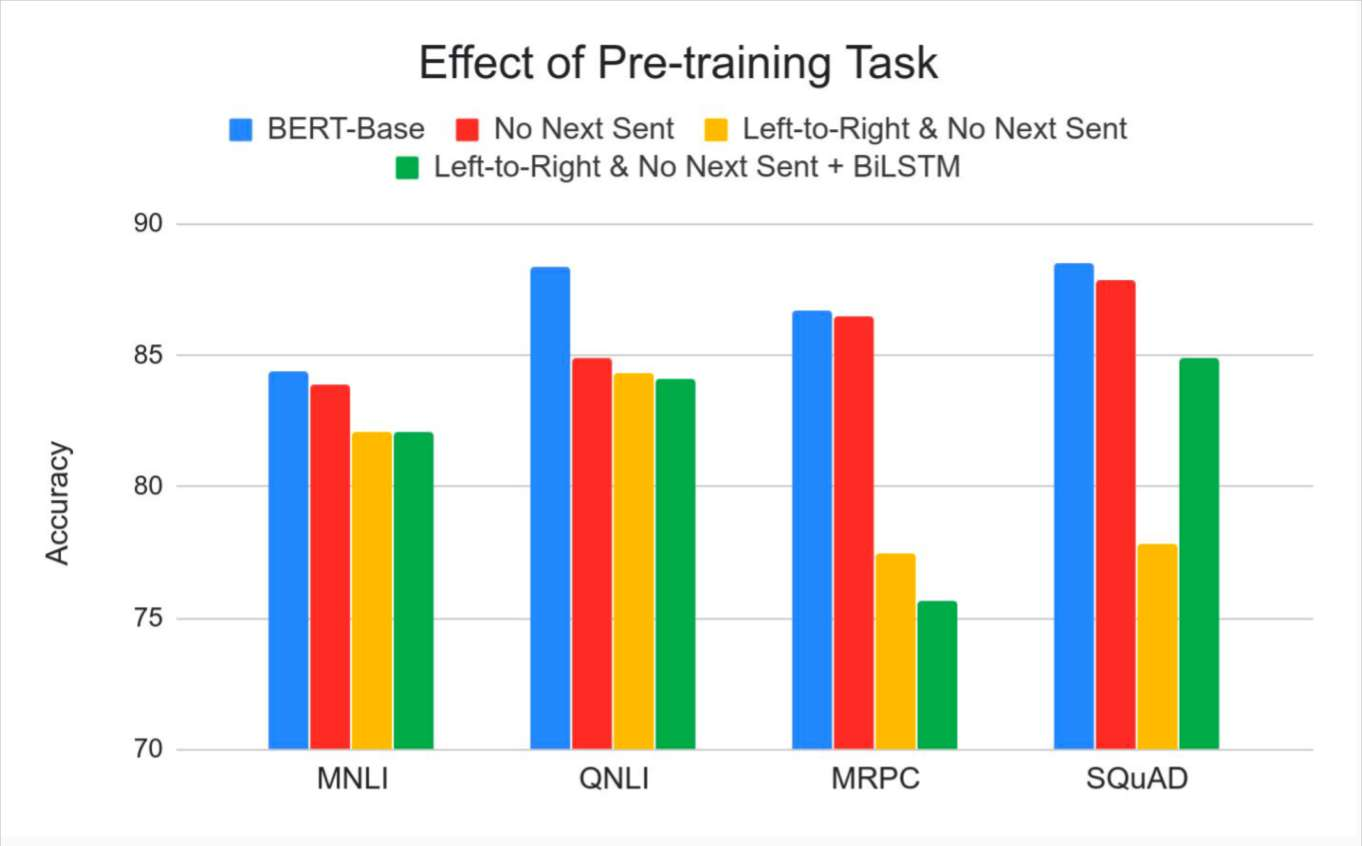
\includegraphics[scale=0.2]{pics/BERTeffect.png}
  \caption{Efecto de la tarea de preentrenamiento en BERT}
\end{figure}

\section{Decodificadores de preentrenamiento GPT y GPT-2}

\begin{itemize}
\item De manera contemporánea a BERT, OpenAI presentó un enfoque alternativo llamado Generative Pretrained Transformer (GPT) \cite{radford2018improving}.
\item La idea detrás de GPT es entrenar un gran modelo de lenguaje estándar utilizando la parte generativa del Transformer, específicamente el decodificador.
\item GPT es un decodificador Transformer con 12 capas y 117 millones de parámetros.
\item Tiene estados ocultos de 768 dimensiones y capas ocultas de avance feed-forward de 3072 dimensiones.
\item GPT utiliza codificación de pares de bytes con 40,000 fusiones para manejar unidades de subpalabras.
\item GPT fue entrenado en BooksCorpus, que consta de más de 7,000 libros únicos.
\item Posteriormente, OpenAI presentó GPT-2, una versión más grande con 1.5 mil millones de parámetros, entrenada con aún más datos.
\item Se ha demostrado que GPT-2 genera muestras relativamente convincentes de lenguaje natural.
\end{itemize}

\paragraph{Salida del modelo GPT-2 (seleccionada)}
\textbf{Inicio proporcionado por un humano}:

En un descubrimiento impactante, los científicos descubrieron una manada de unicornios viviendo en un valle remoto previamente inexplorado, en las montañas de los Andes. Aún más sorprendente para los investigadores fue el hecho de que los unicornios hablaban un inglés perfecto. \\
\textbf{Completado del modelo}:

Los científicos nombraron a la población, debido a su distintivo cuerno, Unicornio de Ovidio. Estos unicornios plateado-blancos de cuatro cuernos eran desconocidos previamente para la ciencia.

Ahora, después de casi dos siglos, el misterio de lo que desencadenó este fenómeno peculiar finalmente se resuelve.

El Dr. Jorge Pérez, un biólogo evolutivo de la Universidad de La Paz, y varios compañeros, estaban explorando las montañas de los Andes cuando encontraron un pequeño valle, sin otros animales ni humanos. Pérez notó que el valle tenía lo que parecía ser una fuente natural, rodeada por dos picos de roca y nieve plateada.


\section{¿Qué tipos de cosas aprende el preentrenamiento?}

\begin{itemize}
\item La Universidad de Stanford está ubicada en \_\_\_\_\_, California. [Datos curiosos]
\item Puse el \_\_\_\_\_ tenedor en la mesa. [sintaxis]
\item La mujer cruzó la calle, verificando el tráfico sobre \_\_\_\_\_ hombro. [co-referencia]
 \item Fui al océano para ver los peces, tortugas, focas y \_\_\_\_\_. [semántica léxica/tema]
\item En general, el valor que obtuve de las dos horas viéndolo fue la suma total de las palomitas de maíz y la bebida. La película fue \_\_\_\_\_. [sentimiento]
\item Iroh entró en la cocina para preparar un poco de té. De pie junto a Iroh, Zuko reflexionó sobre su destino. Zuko dejó el \_\_\_\_\_. [algún razonamiento - esto es más difícil]
\item Estaba pensando en la secuencia que va 1, 1, 2, 3, 5, 8, 13, 21, \_\_\_\_\_ [aritmética básica; no aprenden la secuencia de Fibonacci]
\end{itemize}


\section{Cambio de fase: GPT-3 (2020)}
\begin{itemize}
\item GPT-3 es otro modelo de lenguaje basado en Transformer (LM) que empujó los límites con casi 200 mil millones de parámetros, convirtiéndolo en el modelo más grande en ese momento \cite{brown2020language}.
\item Fue entrenado en un corpus masivo que consiste en casi 500 mil millones de palabras.
\item \textbf{Aprendizaje en contexto}: GPT-3 demostró la capacidad de resolver varias tareas de procesamiento del lenguaje natural (NLP) utilizando \textbf{aprendizaje sin ejemplos}, \textbf{aprendizaje con un solo ejemplo} y \textbf{aprendizaje con pocos ejemplos}.
\item La clave de esta capacidad reside en la instrucción o contexto proporcionado a GPT-3.
\item GPT-3 demostró la capacidad de resolver diversas tareas sin realizar actualizaciones de gradiente en el modelo base.
\end{itemize}

 \begin{figure}[h]
        	
\includegraphics[scale = 0.08]{pics/gpt3.png}
        \end{figure}




\section{Aprendizaje sin ejemplos, con un solo ejemplo y con pocos ejemplos con GPT-3}
GPT-3, uno de los modelos más destacados en el campo de los Modelos de Lenguaje Grandes (LLMs), ha demostrado la capacidad de realizar tareas de procesamiento de lenguaje natural (NLP) mediante aprendizaje sin ejemplos (zero-shot learning), aprendizaje con un solo ejemplo (one-shot learning) y aprendizaje con unos pocos ejemplos (few-shot learning).

En el aprendizaje sin ejemplos, GPT-3 es capaz de abordar tareas sin ningún entrenamiento específico. Esto se logra proporcionando al modelo un prompt o una instrucción que guíe su proceso de generación. Por ejemplo, al proporcionarle una instrucción como "Traduce esta oración en inglés al francés", GPT-3 puede generar la oración traducida sin necesidad de un entrenamiento explícito para tareas de traducción.

En el aprendizaje con un solo ejemplo, GPT-3 puede realizar una tarea al agregar un solo par de entrada-salida a la instrucción. Por ejemplo, si se le proporciona un solo ejemplo de una pregunta y su respuesta, GPT-3 puede generar respuestas coherentes a preguntas similares.

En el aprendizaje con unos pocos ejemplos, se sigue una idea similar a la del aprendizaje con un solo ejemplo, pero proporcionando un número limitado de pares de entrada-salida después de la instrucción en el prompt. Estos ejemplos adicionales ayudan a GPT-3 a generalizar y mejorar su capacidad para abordar la tarea específica.

Estos enfoques de aprendizaje permiten que GPT-3 realice tareas de procesamiento de lenguaje natural sin necesidad de entrenamiento intensivo en cada tarea específica. Esto ha abierto nuevas posibilidades en el desarrollo de aplicaciones de NLP y ha demostrado el poder de los Modelos de Lenguaje Grandes en la resolución de diversas tareas de lenguaje.


 \begin{figure}[h]
        	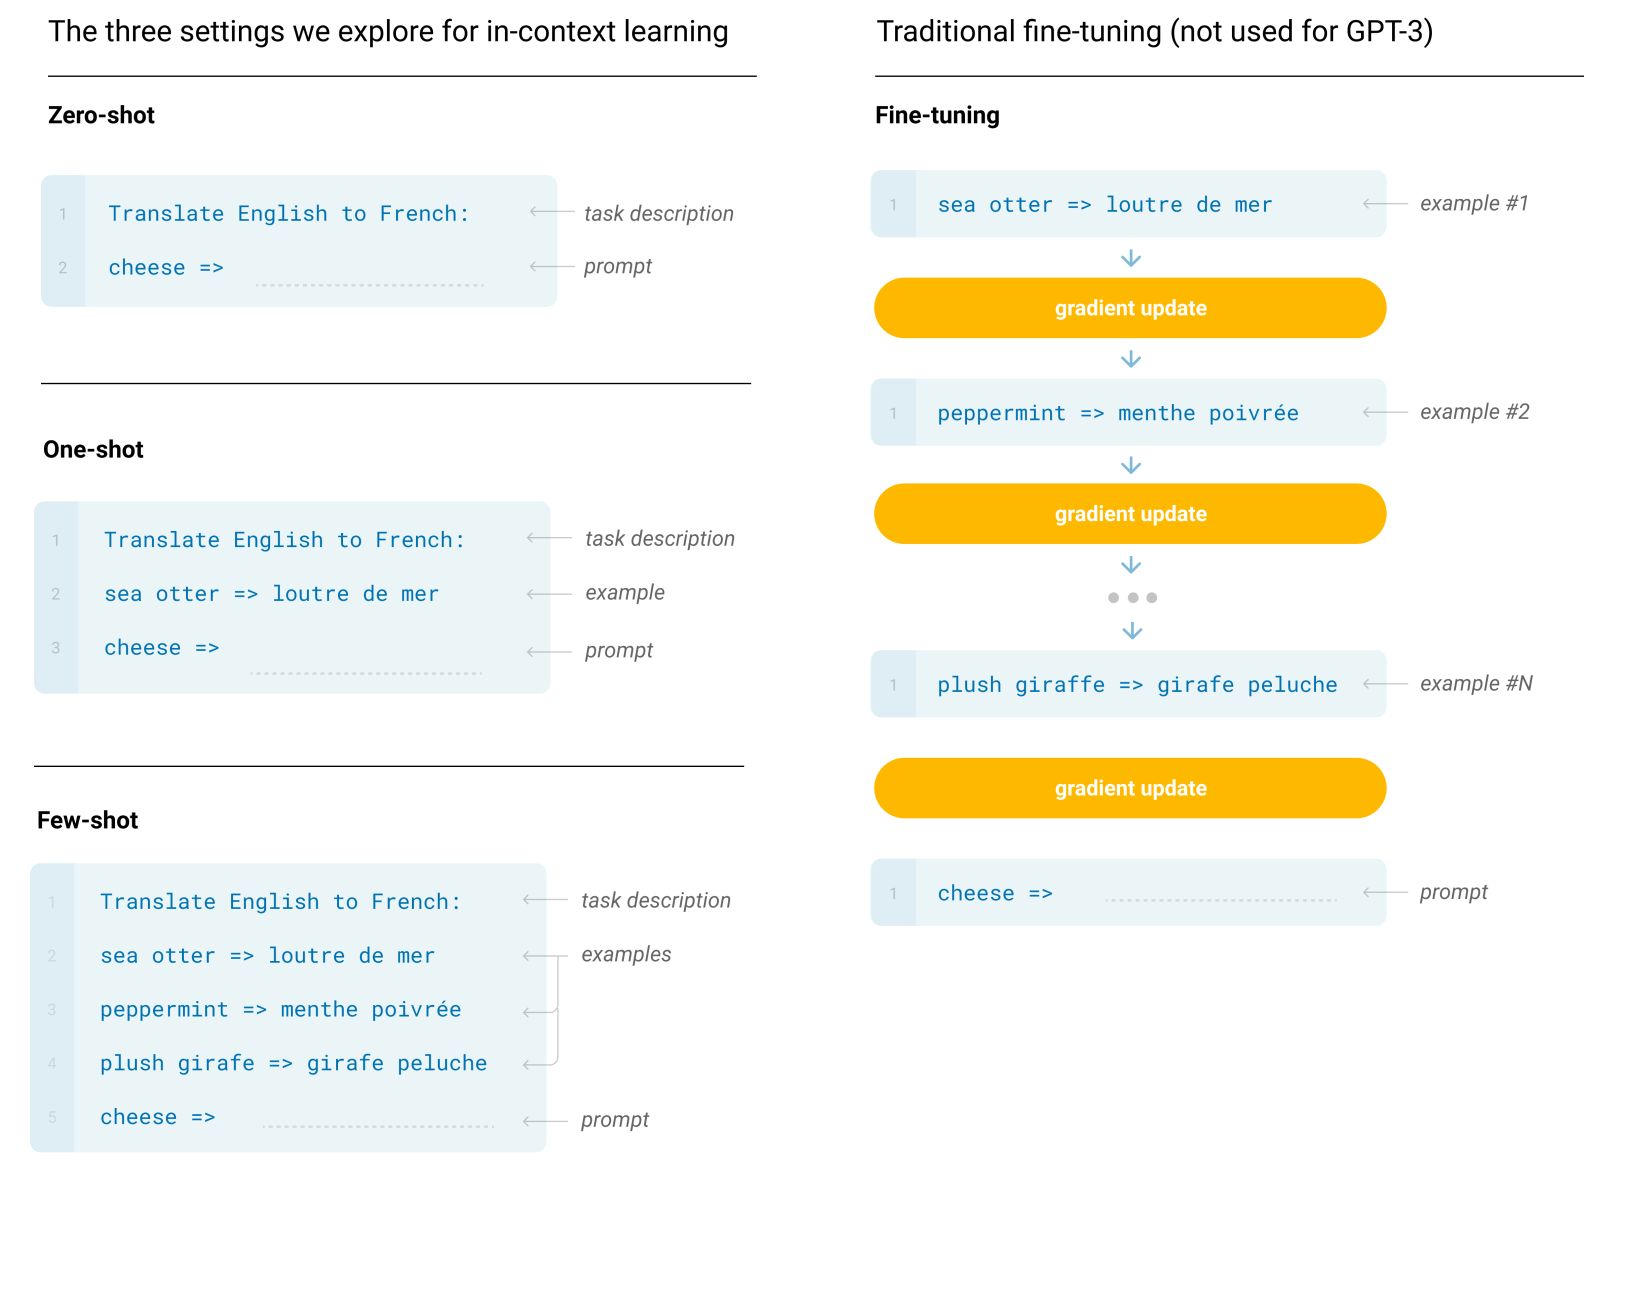
\includegraphics[scale = 0.18]{pics/zeroonefew.png}
        \end{figure}



GPT-3 Resultados en Few-shot learning
 \begin{figure}[h]
        	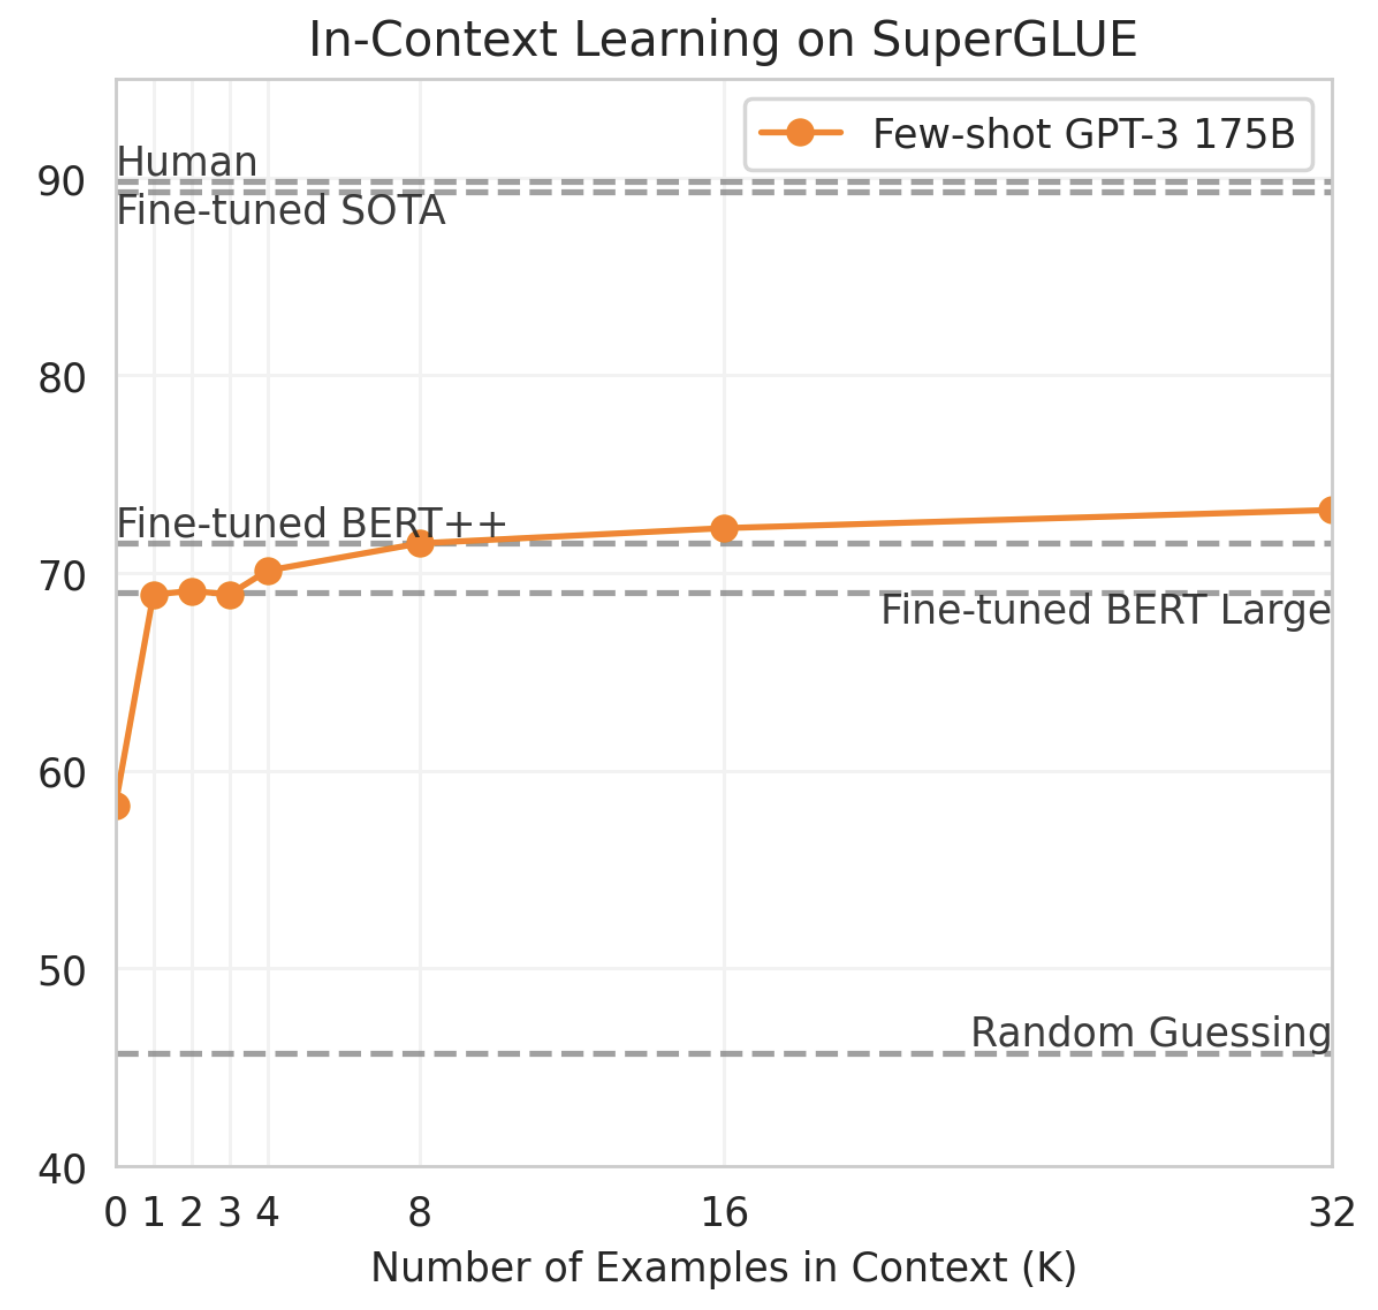
\includegraphics[scale = 0.15]{pics/fewshotresults.png}
        \end{figure}



\section{Chain-of-thought Prompting}
Chain-of-thought prompting es un mecanismo simple para provocar un comportamiento de razonamiento de múltiples pasos en modelos de lenguaje grandes.

La idea detrás de chain-of-thought prompting es ampliar cada ejemplo en el prompt de few-shot learning con una cadena de pensamiento asociada a la respuesta. En lugar de proporcionar solo un par de entrada-salida, se agrega un contexto adicional que guía al modelo a través de una serie de pasos de razonamiento \cite{wei2022chain}.

Por ejemplo, en lugar de simplemente proporcionar un ejemplo de pregunta y respuesta, se puede agregar una cadena de pensamiento que muestra cómo se llega a la respuesta paso a paso. Esto ayuda a los modelos de lenguaje a comprender mejor el proceso de razonamiento requerido para abordar la tarea.

La idea detrás de chain-of-thought prompting es mejorar la capacidad de los modelos de lenguaje para realizar razonamientos más sofisticados y responder a preguntas que requieren múltiples pasos de inferencia. Al proporcionar un contexto más detallado y explicativo en el prompt, se espera que los modelos puedan generar respuestas más completas y coherentes.

Chain-of-thought prompting es una técnica prometedora que puede mejorar la capacidad de los modelos de lenguaje para realizar razonamientos complejos y abordar tareas de procesamiento de lenguaje natural que requieren múltiples pasos de inferencia. Su aplicación puede ampliar las capacidades de los modelos y permitir su uso en una variedad más amplia de aplicaciones de NLP.

 \begin{figure}[h]
        	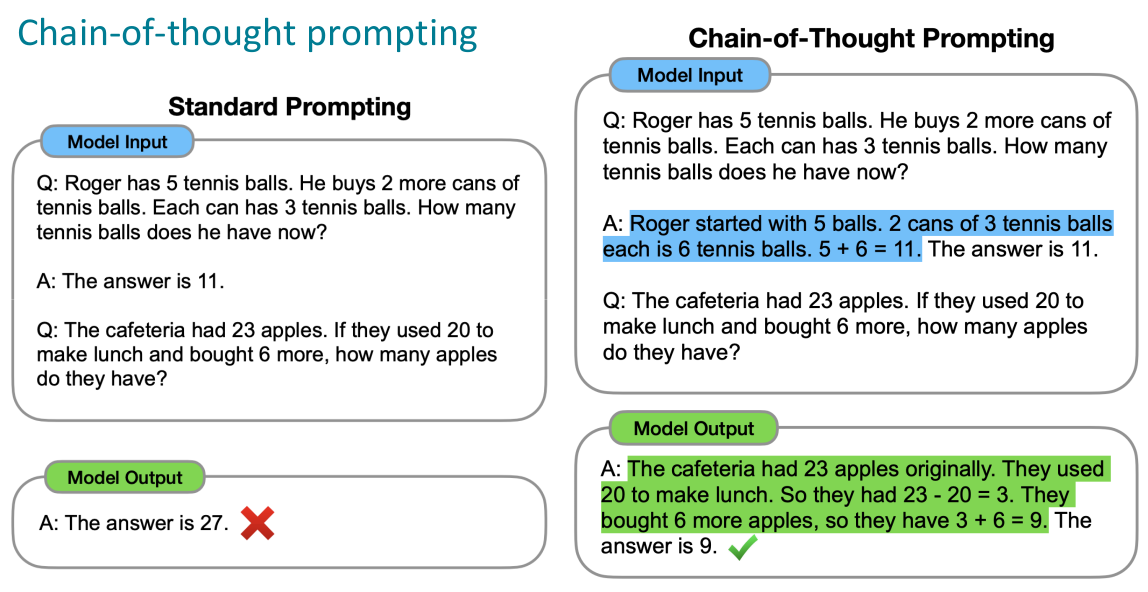
\includegraphics[scale = 0.3]{pics/chainoftought.png}
        \end{figure}



\section{Modelos de Lenguaje como Asistentes de Usuario (o Chatbots)}
Los Modelos de Lenguaje Grandes (LLMs) han demostrado ser herramientas poderosas para interactuar con los usuarios y actuar como asistentes de usuario o chatbots. Sin embargo, los LLMs autoregresivos no están alineados directamente con la intención del usuario y pueden generar respuestas que no cumplen con las expectativas.

Un problema común con los LLMs autoregresivos es que pueden producir respuestas vagas, repetitivas o poco relevantes para las consultas de los usuarios. Esto se debe a la naturaleza generativa del modelo, que puede generar texto sin una comprensión profunda de la intención del usuario o el contexto de la conversación.

Una solución a este problema es el ajuste fino de los modelos de lenguaje para alinearlos con la intención del usuario. El ajuste fino implica entrenar el modelo en un conjunto de datos específico para mejorar su capacidad de generar respuestas relevantes y coherentes.

 \begin{figure}[h]
        	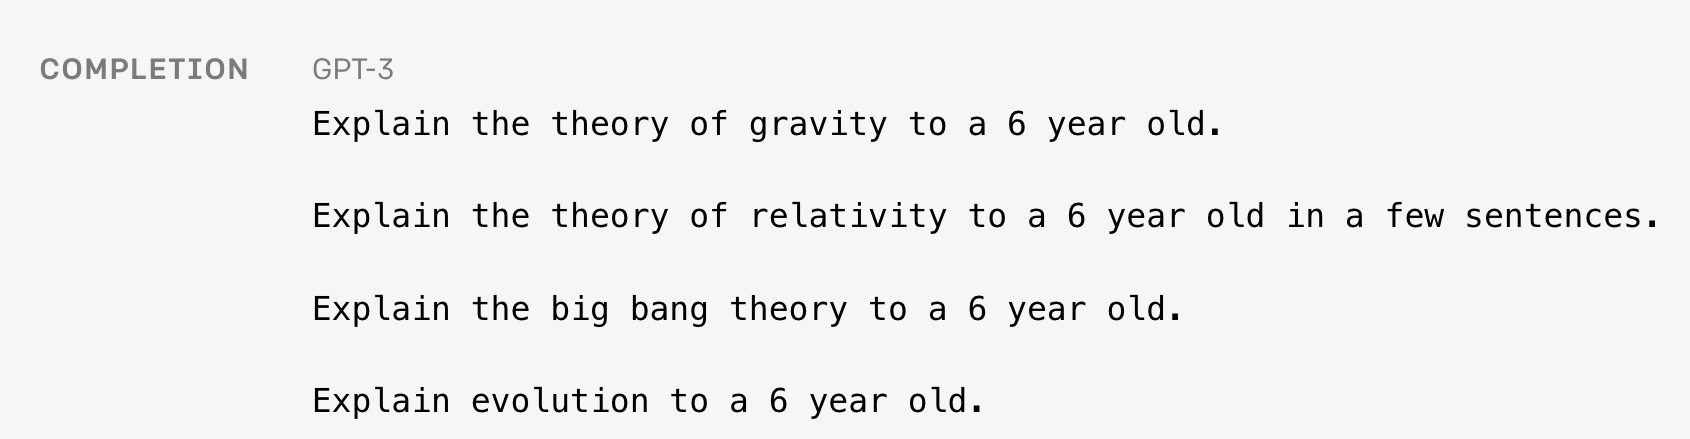
\includegraphics[scale = 0.34]{pics/lmnotuserassistant.png}
        \end{figure}

\subsection{LaMDA: Modelos de Lenguaje para Aplicaciones de Diálogo}
LaMDA es un modelo de lenguaje desarrollado por Google basado en el Transformer, optimizado para diálogos en dominio abierto \cite{thoppilan2022lamda}. Este modelo cuenta con 137 mil millones de parámetros y se entrena con 1.56 mil millones de palabras.

El proceso de entrenamiento de LaMDA es similar al de los modelos de lenguaje tradicionales, donde se realiza un pre-entrenamiento para predecir palabras. Sin embargo, LaMDA se enfoca especialmente en datos de diálogos durante el pre-entrenamiento. Posteriormente, el modelo se ajusta finamente para generar respuestas teniendo en cuenta varios criterios.

Para lograr que LaMDA cumpla con todos estos criterios, se trabajó con un gran número de trabajadores de la multitud. Estas personas etiquetaron manualmente las conversaciones a partir del modelo pre-entrenado.

\begin{figure}[h]
	\centering
	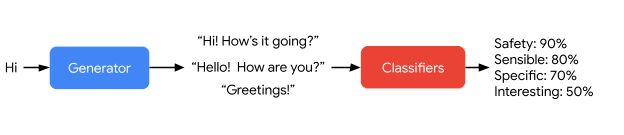
\includegraphics[scale = 0.5]{pics/lambda.png}
	\caption{Arquitectura del modelo de lenguaje LaMDA.}
\end{figure}

El desarrollo de LaMDA se centró en cumplir con los siguientes criterios de optimización:

\paragraph{Criterios de Optimización de LaMDA}

\textbf{Calidad}
\begin{itemize}
\item Sensatez: proporcionar respuestas significativas.
\item Especificidad: evitar respuestas vagas.
\item Interesante: proporcionar respuestas perspicaces, inesperadas o ingeniosas.
\end{itemize}

\textbf{Seguridad}
\begin{itemize}
\item Evitar lenguaje violento.
\item Evitar discursos de odio.
\item Evitar discursos estereotipados.
\end{itemize}

\textbf{Basamento e Informatividad}
\begin{itemize}
\item Evitar proporcionar respuestas no validadas por fuentes externas.
\item Optimizar la fracción de respuestas que pueden ser validadas en fuentes autorizadas mediante el uso de motores de búsqueda.
\end{itemize}

LaMDA ha sido evaluado comparándolo con el modelo pre-entrenado original y con juicios humanos. Para llevar a cabo la evaluación, se empleó a un grupo independiente de personas que respondieron cuestionarios específicos.

\begin{figure}[h]
	\centering
	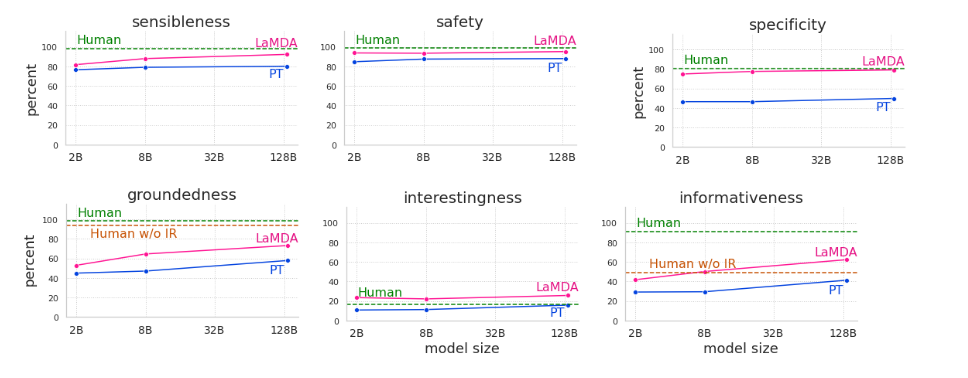
\includegraphics[scale = 0.45]{pics/lambdaresults.png}
	\caption{Resultados de la evaluación de LaMDA.}
\end{figure}

Los resultados de la evaluación demuestran la mejora lograda con LaMDA en comparación con el modelo pre-entrenado original. El enfoque en los criterios de calidad, seguridad, basamento e informatividad ha permitido que LaMDA genere respuestas más precisas y relevantes en diálogos de dominio abierto.

\subsection{ChatGPT y RLHF}
ChatGPT es un modelo desarrollado por OpenAI, similar a LaMDA, que también se centra en aplicaciones de diálogo. Fue lanzado a finales de 2022 y utiliza un enfoque de colaboración masiva para mejorar sus respuestas. Sin embargo, a diferencia de LaMDA, ChatGPT utiliza el Aprendizaje por Refuerzo a partir de Retroalimentación Humana (RLHF) en su proceso de ajuste fino \cite{ouyang2022training}.

El Aprendizaje por Refuerzo (RL) es un paradigma de aprendizaje automático en el que un agente aprende a tomar decisiones en un entorno para maximizar una recompensa acumulativa. En el caso de ChatGPT, el modelo se ajusta finamente mediante RLHF utilizando una función de preferencia que asigna una puntuación a las respuestas generadas y ajusta el modelo de lenguaje en consecuencia.

El proceso de RLHF implica la recopilación de muestras de interacciones entre el modelo y los usuarios reales. Estas muestras son utilizadas para entrenar un modelo de clasificación que asigna una puntuación a las respuestas generadas. El modelo de lenguaje se ajusta entonces utilizando algoritmos de optimización por refuerzo para maximizar la recompensa esperada.

El enfoque RLHF tiene como objetivo mejorar la calidad y la relevancia de las respuestas generadas por ChatGPT al guiar el ajuste fino del modelo con la ayuda de la retroalimentación humana. Este proceso iterativo de ajuste y retroalimentación ayuda a refinar las respuestas del modelo y alinearlas mejor con las expectativas de los usuarios.

\begin{figure}[h]
	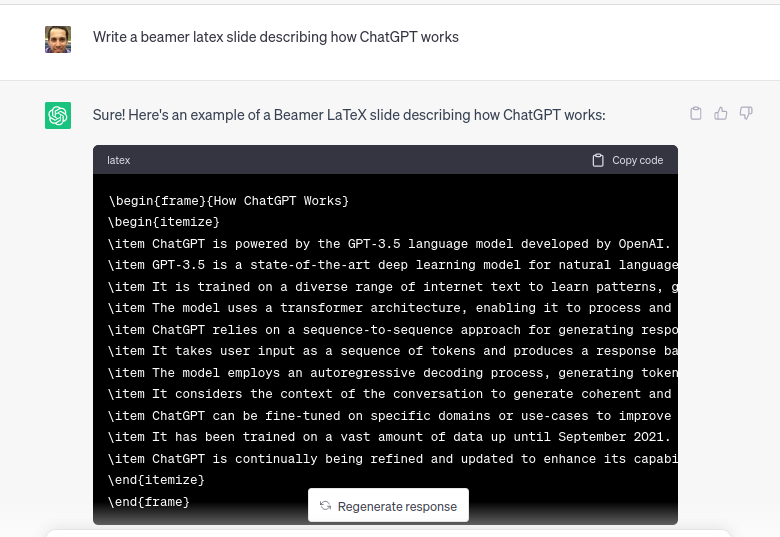
\includegraphics[scale = 0.25]{pics/chatgpt.png}
\end{figure}

 \begin{figure}[h]
        	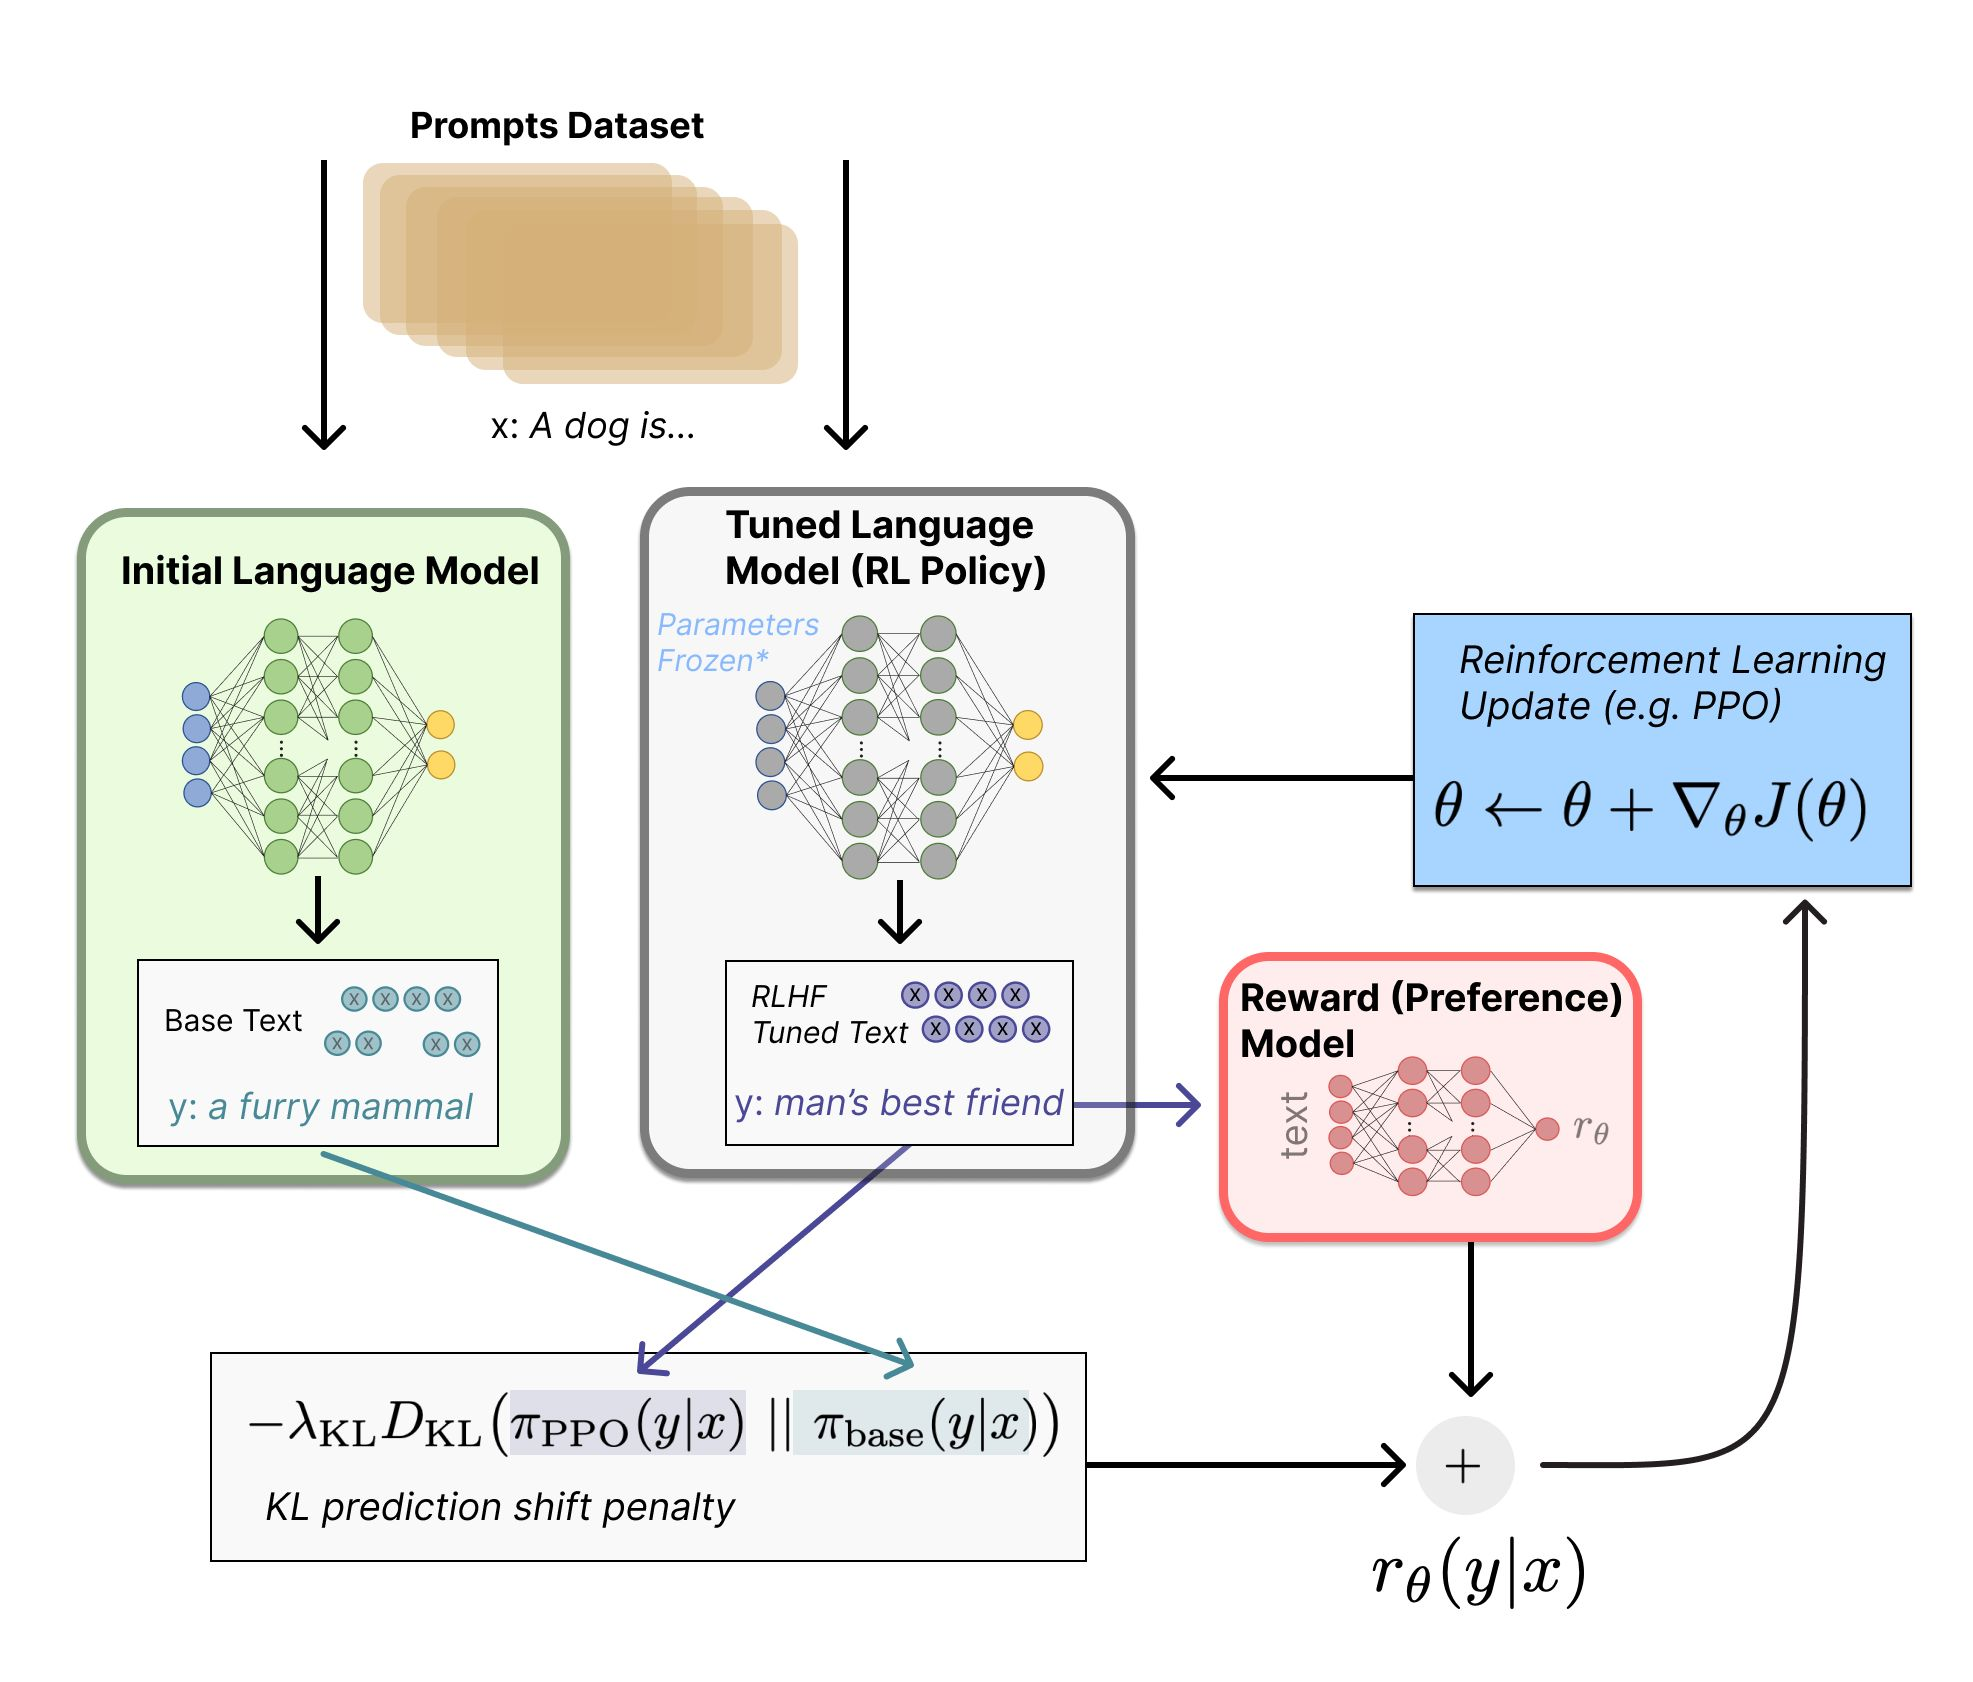
\includegraphics[scale = 0.12]{pics/RLHF.png}
        \end{figure}
        Source: \url{https://huggingface.co/blog/rlhf}



\subsection{GPT-4 (2023)}
GPT-4 \cite{openai2023gpt4} es el último modelo de lenguaje desarrollado por OpenAI. Fue lanzado en 2023 y representa una evolución significativa en comparación con sus predecesores. Una de las principales características de GPT-4 es su capacidad para incluir imágenes como parte de las instrucciones o el contexto de entrada.

GPT-4 sigue siendo un modelo de lenguaje basado en la arquitectura Transformer, pero con mejoras en la capacidad de procesamiento y generación de texto en combinación con imágenes. Esta mejora permite a GPT-4 comprender y responder a consultas que involucran información visual, como preguntas sobre el contenido de una imagen o la descripción de elementos visuales específicos.

Un aspecto destacado de GPT-4 es su capacidad para aprobar exámenes en varias disciplinas. Al poder procesar las imágenes asociadas con las preguntas, GPT-4 puede generar respuestas precisas y detalladas basadas tanto en información textual como visual.

Es importante destacar que, a partir de ChatGPT y GPT-4, las empresas han dejado de hacer públicos todos los detalles de la construcción de sus modelos.

\begin{figure}[h]
	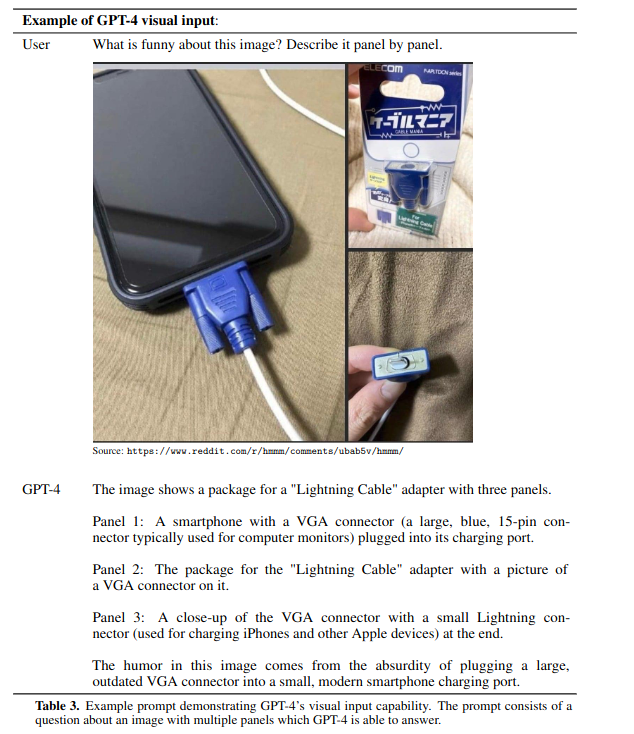
\includegraphics[scale = 0.35]{pics/gpt4.png}
\end{figure}




\section{Ajuste Fino de Instrucciones}
Una forma más eficiente de ajustar los Modelos de Lenguaje Grandes (LLMs) es mediante el ajuste fino de instrucciones \cite{chung2022scaling}. Este enfoque consiste en recopilar ejemplos de pares (instrucción, salida) para diversas tareas y ajustar el LLM en base a estos ejemplos.

La idea detrás del ajuste fino de instrucciones es utilizar ejemplos de instrucciones y las salidas esperadas correspondientes para enseñar al LLM a realizar tareas específicas de manera más precisa. Al recopilar una amplia variedad de ejemplos de diferentes tareas, se puede mejorar la capacidad del modelo para comprender y generar respuestas relevantes y coherentes.

Una vez que se ha realizado el ajuste fino de las instrucciones, se evalúa el rendimiento del modelo en tareas no vistas previamente. Esto permite medir la generalización del modelo y su capacidad para abordar nuevas tareas más allá de las utilizadas durante el ajuste fino.

El ajuste fino de instrucciones es un enfoque prometedor para mejorar la eficiencia del ajuste fino en los LLMs. Al recopilar ejemplos de instrucciones y salidas esperadas en lugar de realizar ajustes finos en cada tarea por separado, se ahorra tiempo y recursos computacionales.

\section{Línea de tiempo de los Modelos de Lenguaje Grandes}
A día de hoy (2023), el desarrollo de nuevos Modelos de Lenguaje Grandes continúa sin interrupciones. Estos modelos han experimentado un crecimiento y avance acelerado en los últimos años, superando constantemente los límites anteriores en términos de tamaño y capacidad.

La siguiente es una línea de tiempo que muestra algunos de los modelos de lenguaje grandes existentes en los últimos años, que tienen un tamaño superior a los 10 mil millones de parámetros \cite{zhao2023survey}. Esta línea de tiempo destaca los avances significativos que se han logrado en este campo y cómo los modelos han evolucionado a lo largo del tiempo.

\begin{figure}[h]
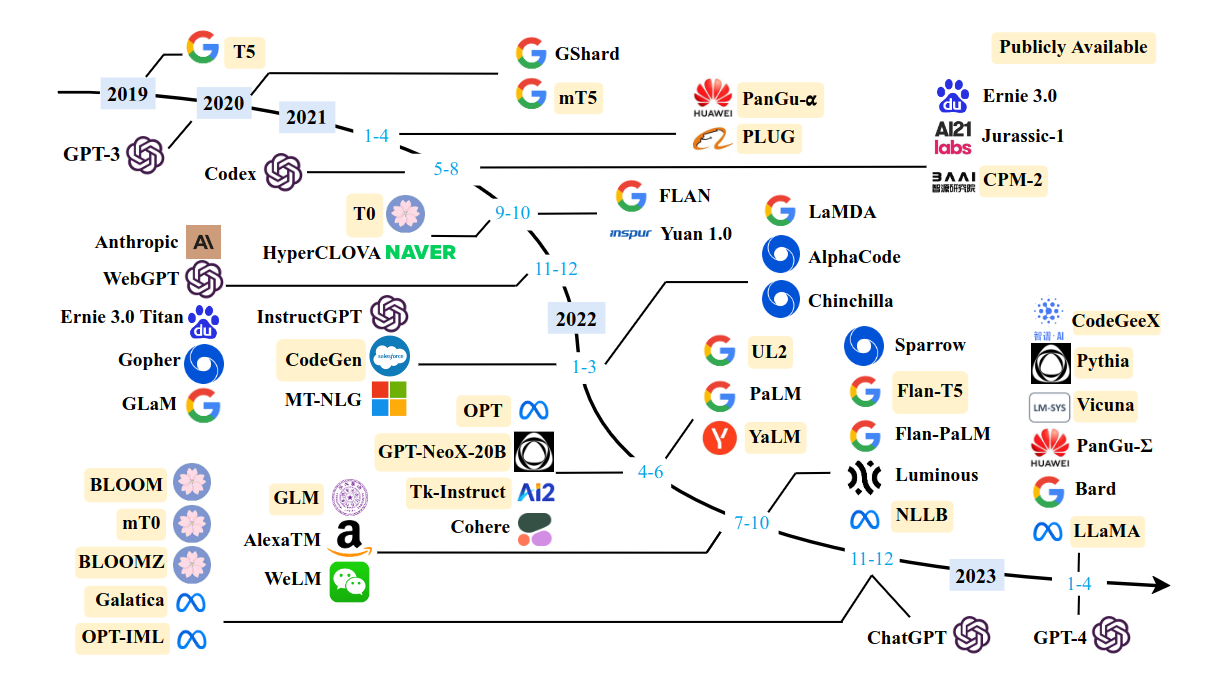
\includegraphics[scale = 0.33]{pics/llmtimeline.png}
\end{figure}



\section{Prompt Engineering}
La ingeniería de prompts es una nueva disciplina para desarrollar y optimizar prompts que aprovechen eficientemente los modelos de lenguaje (LMs). Consiste en diseñar instrucciones o contextos específicos para guiar el comportamiento de los modelos y obtener resultados deseados.

En el caso de los modelos de lenguaje generativos, como GPT-3, el prompt es crucial para influir en la generación de texto. Un prompt bien diseñado puede ayudar a obtener respuestas más precisas y coherentes, alineadas con la intención del usuario.

Existen diferentes técnicas de ingeniería de prompts. Algunas estrategias comunes incluyen:
\begin{itemize}
\item \textbf{Prompt priming}: proporcionar un contexto inicial que establezca el tema o la dirección de la conversación. Por ejemplo, si se desea obtener información sobre el clima en una ubicación específica, el prompt podría comenzar con "Dime cómo estará el clima en".
\item \textbf{Prompt expansion}: ampliar el prompt con información adicional o detalles relevantes para obtener respuestas más precisas. Por ejemplo, si se busca información sobre un libro, se podría incluir el título, el autor y el género en el prompt.
\item \textbf{Prompt rewriting}: reformular el prompt para hacerlo más claro y específico. Esto puede implicar simplificar la pregunta, eliminar ambigüedades o especificar los detalles requeridos.
\item \textbf{Prompt combination}: combinar múltiples prompts o preguntas en una sola para obtener respuestas más completas o enriquecedoras. Esto puede ser útil cuando se busca información detallada sobre un tema específico.
\end{itemize}

La ingeniería de prompts es un proceso iterativo que requiere experimentación y ajustes para lograr los resultados deseados. Es importante comprender el comportamiento del modelo y cómo responde a diferentes tipos de prompts para obtener los mejores resultados.

 \begin{figure}[h]
        	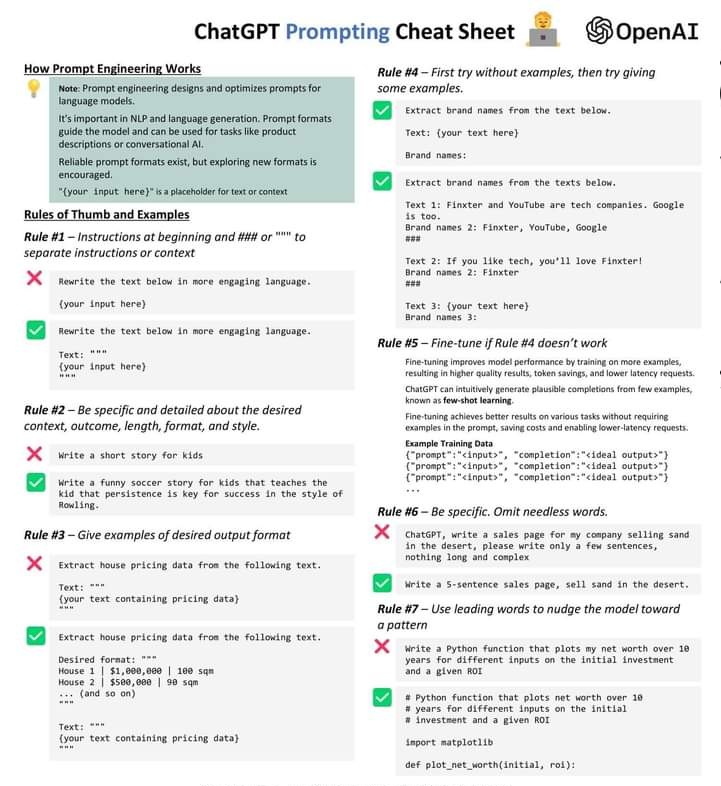
\includegraphics[scale = 0.33]{pics/prompting.png}
        \end{figure}


\section{Peligros de los Grandes Modelos de Lenguaje}
A medida que los Modelos de Lenguaje Grandes (LLMs) continúan evolucionando y volviéndose más poderosos, la comunidad de investigación ha planteado preocupaciones sobre varios peligros asociados a estos modelos \cite{bender2021dangers}.

\begin{itemize}
\item \textbf{Alucinación}: Los modelos de lenguaje probabilísticos pueden generar información fabricada sin una base factual. Esto significa que pueden generar respuestas que no están respaldadas por datos verificables o información precisa.

\item \textbf{Equidad}: Los LLMs pueden perpetuar los sesgos presentes en los datos de entrenamiento, lo que incluye lenguaje tóxico, racismo y discriminación de género. Estos sesgos pueden llevar a respuestas sesgadas y perjudiciales para ciertos grupos de personas.

\item \textbf{Infracción de derechos de autor}: Los LLMs grandes pueden violar las leyes de derechos de autor al reproducir contenido sin la autorización adecuada. Esto plantea preocupaciones legales y éticas en relación con la propiedad intelectual.

\item \textbf{Falta de transparencia}: La naturaleza compleja de los LLMs dificulta la interpretación de sus predicciones y el entendimiento del razonamiento detrás de respuestas específicas. Esto puede generar desconfianza en los resultados y dificultar la rendición de cuentas.

\item \textbf{Monopolización}: El costo alto de entrenar estos modelos crea barreras para que las empresas que no son de tecnología puedan competir en el mismo nivel. Esto puede llevar a una concentración de poder en manos de unas pocas grandes empresas de tecnología.

\item \textbf{Huella de carbono elevada}: El proceso de entrenamiento intensivo en energía de los LLMs contribuye a una huella de carbono significativa. Esto plantea preocupaciones sobre el impacto ambiental y la sostenibilidad de estos modelos a gran escala.

Estas preocupaciones resaltan la importancia de abordar los desafíos éticos, legales y sociales asociados con los LLMs. Se necesita una regulación adecuada, transparencia en la investigación y desarrollo, y enfoques responsables para garantizar que los LLMs se utilicen de manera ética y beneficiosa para la sociedad en general.
\end{itemize}

\section{Conclusiones}
El crecimiento en tamaño y potencia de los Modelos de Lenguaje Grandes ha acelerado de manera significativa en los últimos años. Estos modelos han demostrado capacidades impresionantes en diversas tareas de procesamiento de lenguaje natural y han abierto nuevas posibilidades en áreas como la generación de texto, la traducción automática, los chatbots y mucho más.

A medida que avanzamos, es difícil predecir con certeza qué nos deparará el futuro en términos de desarrollo de modelos de lenguaje. Sin embargo, hay algunas tendencias que se pueden anticipar con confianza.

En primer lugar, es probable que veamos una proliferación de modelos generativos para diversos formatos, como texto, código, imágenes, video y realidades virtuales. Los Modelos de Lenguaje Grandes seguirán siendo el centro de atención en la generación de contenido en estos formatos.

Además, habrá una gran cantidad de agentes y programas que interactuarán y tomarán decisiones basadas en la interacción con estos modelos. Esto podría incluir asistentes médicos, programas de inversión, agentes de viajes y muchos otros sistemas que utilizan modelos de lenguaje para comprender y responder a las necesidades de los usuarios.

Si bien los avances en los Modelos de Lenguaje Grandes son emocionantes, también es importante abordar los desafíos y peligros asociados. Es fundamental tener en cuenta la ética, la transparencia, la equidad y la sostenibilidad al desarrollar y utilizar estos modelos para garantizar que se beneficien a todos los usuarios y la sociedad en general.





